\documentclass{article}

\usepackage{amssymb}
\usepackage{tikz}
\usetikzlibrary{positioning}

\title{Interaction Diagram - Tag Book}
\author{Nicholas Riesen}

% no page number at bottom
\pagenumbering{gobble}

\begin{document}
\maketitle

\begin{center}
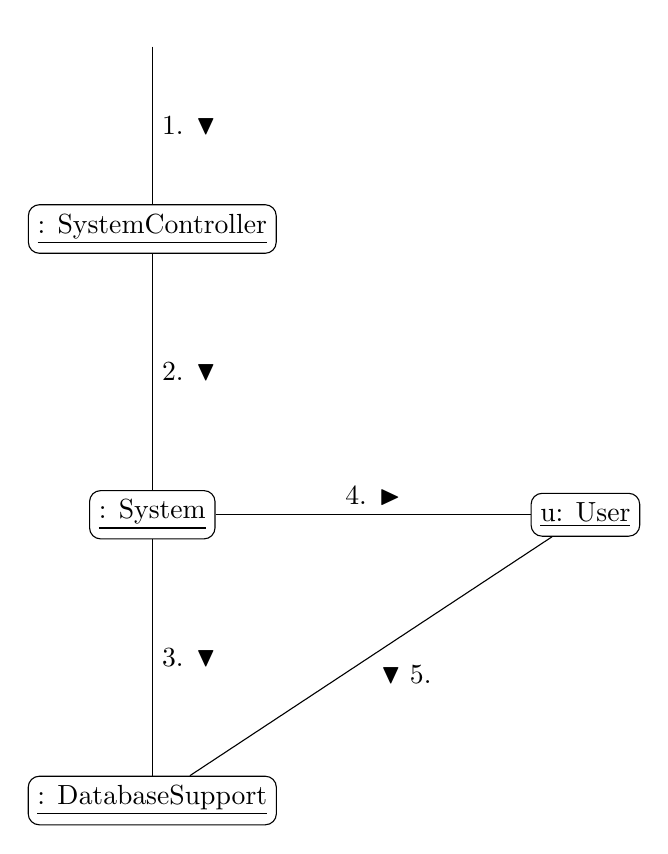
\begin{tikzpicture}[
  auto,
  block/.style = {
    rectangle,
    draw=black,
    align=center,
    rounded corners
  }
]

\node[] (start)  {};

\node[block, below = 2cm of start]      (controller) {\underline{: SystemController}};
\node[block, below = 3cm of controller] (system)     {\underline{: System}}; 
\node[block, right = 4cm of system]     (user)       {\underline{u: User}};
\node[block, below = 3cm of system]     (database)   {\underline{: DatabaseSupport}};

\draw (start)      -- (controller) node[midway] {1. $\blacktriangledown$};
\draw (controller) -- (system)     node[midway] {2. $\blacktriangledown$};
\draw (system)     -- (database)   node[midway] {3. $\blacktriangledown$};
\draw (system)     -- (user)       node[midway] {4. $\blacktriangleright$};
\draw (user)       -- (database)   node[midway] {$\blacktriangledown$ 5.};

\end{tikzpicture}
\end{center}

\vspace{0.5cm}

\begin{enumerate}
  \item \texttt{b:=addTag(uid:String, bookTitle:string, tag:string):boolean}
  \item \texttt{b:=addTag(uid:String, bookTitle:string, tag:string):boolean}
  \item \texttt{u:=getUser(uid:String):User}
  \item \texttt{b:=addTag(bookTitle:String, tag:String):boolean}
  \item \texttt{5:b:=addTag(uid:string, bookTitle:string, tag:string):boolean}
\end{enumerate}
\end{document}
